\part{Introduction to Programming}

\chapter{Best Practices}
\chapter{Day 6 - Introduction to C++}
\begin{Goals}
\begin{enumerate}
    \item Compile a basic C++ program
    \item Identify sections of source code
    \item Manage input and output in your code
    \item Handle variables, including initialization, assignment, modification, and recall.
    \item Read from and write to files, including parsing/processing inputs and formatting outputs.
\end{enumerate}
\end{Goals}
\paragraph{}C++ is a compiled language, which means that before a program written with it can be executed, it must be compiled from human-readable text into the binary machine language.

By convention, C++ source code files (the text you can read and edit) end with \texttt{.cpp}, compiled object files end in \texttt{.o}, and completed executables end in \texttt{.x}.

The basic compilation command we will be using is below:

\begin{verbatim}
    g++ main.cpp -o output.x
\end{verbatim}

This calls the compiler \texttt{g++} on the source file \texttt{main.cpp}, with the resulting output (\texttt{-o}) as \texttt{output.x}.  The program can then be executed like any other command-line program by calling it with \texttt{./output.x}.

To start, every C++ program will have the following basic structure:

\begin{minted}{c++}
#include <iostream>
#include <cstdlib>
int main()
// single-line comment
{
    std::cout << "Hello World!" << std::endl;
    return 0;
}
/* This is a multi-
line comment between the start and end asterisk-slashes
*/
\end{minted}

Let's break this down into some major pieces.  The first section is where libraries and other required files are included.  In this example, we're including the \texttt{iostream} library, which manages the input/output streams of C++, and \texttt{cstdlib}, the C Standard Library which contains a wide array of commonly used functions.  As we progress, we will encounter more libraries with their own unique usefulness.
\begin{minted}{c++}
#include <iostream>
#include <cstdlib>
\end{minted}

The next section is where the main program loop is written.  It must be called "main" for C++ compilers to understand where the starting point of the program is when it's run.  The datatype \texttt{int} is used by convention to allow for integer-based exit codes to be returned to the operating system.  This is useful for error reporting - if the program fails in a way the programmer has anticipated, it can return a specific integer value to the operating system to alert it to the failure.

The \textbf{scope} of the \texttt{main()} function is defined by the open- and close- curly braces.  Throughout C++, this will be how scope is defined and maintained.  Inside the scope is where all the program's functions and commands are stored.  At the end of any program or function (with a specific exception we will get into later), there \textbf{must be a \texttt{return} command}.  Also note that at the end of every command line, there is a semicolon.
\begin{minted}{c++}
int main()
{
    std::cout << "Hello World!" << std::endl;
    return 0;
}
\end{minted}

\section{Version Control, Git, and GitHub}
Version control is a critically important habit to develop early on.
In the simplest form, version control provides a means of keeping track of the changes you've made to your code as you go, as well as providing information about who made which changes in a collaborative project.
More complicated version control can lead to things like software written for different types of hardware, or for different scales of calculations, etc.
Many of us have used version control at some point in our educations, whether we realized it or not.
How many times have you had a document labelled "Document\_v2\_Final\_FINAL\_FINAL\_v3"?
That is an example (albeit not the greatest) of version control.
Keeping track of changes made and versions of your code can be a way to safeguard your work against potential losses and help you track down the source of bugs and errors that may arise.


The most commonly used tool for version control is \texttt{git}, with related websites \href{https://www.github.com}{GitHub}, \href{https://about.gitlab.com/}{GitLab}, and \href{https://bitbucket.org/}{Bitbucket}. 
For the purposes of this workshop, we'll focus on using GitHub because it's free and most (if not all) of us already have accounts there.

There are a few steps to do first if you've never used \texttt{git} on your current computer before. 
These will configure your computer for use with your GitHub account. 
If you use multiple computers (including working from a HPC/Supercomputer), these steps will need to be completed for each computer you use.

\begin{center}\rule{0.5\linewidth}{0.5pt}\end{center}

Configure your local machine with an SSH-key. 
This will allow your computer to connect to other \textbf{trusted} computers that you've previously designated as such, and this includes your Github account.

\begin{Shaded}
\begin{Highlighting}[]
    \BuiltInTok{cd} \VariableTok{\$HOME}
    \FunctionTok{ssh{-}keygen}
\end{Highlighting}
\end{Shaded}

will give the following response/prompt:

\begin{verbatim}
    Generating public/private rsa key pair
    Enter file in which to save the key (/home/username/.ssh/id_rsa): 
\end{verbatim}

If the file already exists, choose a new filename such as
\texttt{git\_rsa} or something you'll recognize.

\begin{verbatim}
    Enter passphrase (empty for no passphrase): 
    Enter same passphrase again: 
\end{verbatim}

You can set a passphrase if you want, but keep in mind you'll be
entering it every single time you upload changes of your code to GitHub.
Some people choose not to have a passphrase for this particular aspect
of their work, others do.

\begin{verbatim}
    Your identification has been saved in /home/username/.ssh/git_rsa
    Your public key has been saved in /home/username/.ssh/git_rsa.pub
    The key fingerprint is:
    SHA256:8U9t+r+SwCi8Xe8uu3HCjbHa7WU51A9pArzm9+F+esk username@Computer
    The key's randomart image is:
    +---[RSA 3072]----+
    |                 |
    |       .         |
    |        +  . +   |
    |         =. =. ..|
    |      . S =*o.=..|
    |       = .oBo+..o|
    |        ..o+*o.*.|
    |       . o.+o*D .|
    |           +@Bo*o|
    +----[SHA256]-----+
\end{verbatim}
\begin{center}\rule{0.5\linewidth}{0.5pt}\end{center}
Add the SSH key to your GitHub Account to allow your computer to access
it.

Go to your account settings page and click on
\texttt{SSH\ and\ GPG\ keys}, then click on \texttt{New\ SSH\ key}.

\begin{figure}
\centering
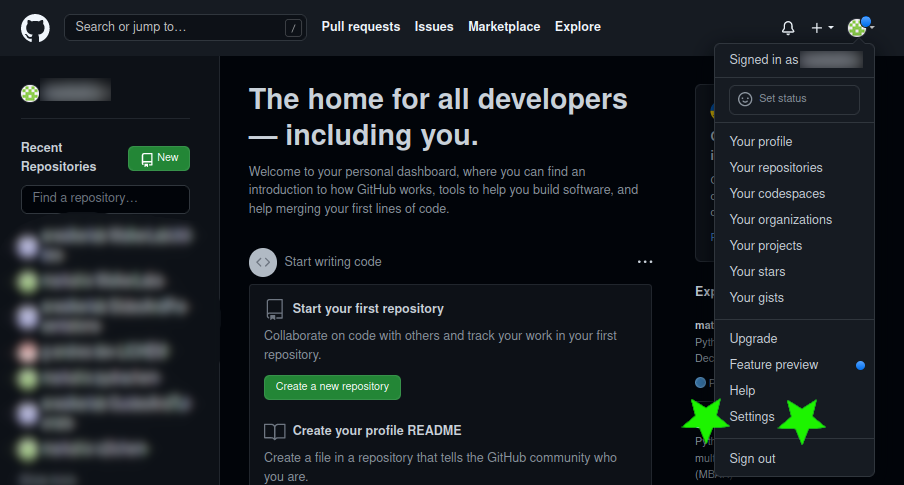
\includegraphics[width=0.8\textwidth]{Images/GH_01.png}
\caption{GitHub Step 1}
\end{figure}
\FloatBarrier

\begin{figure}
\centering
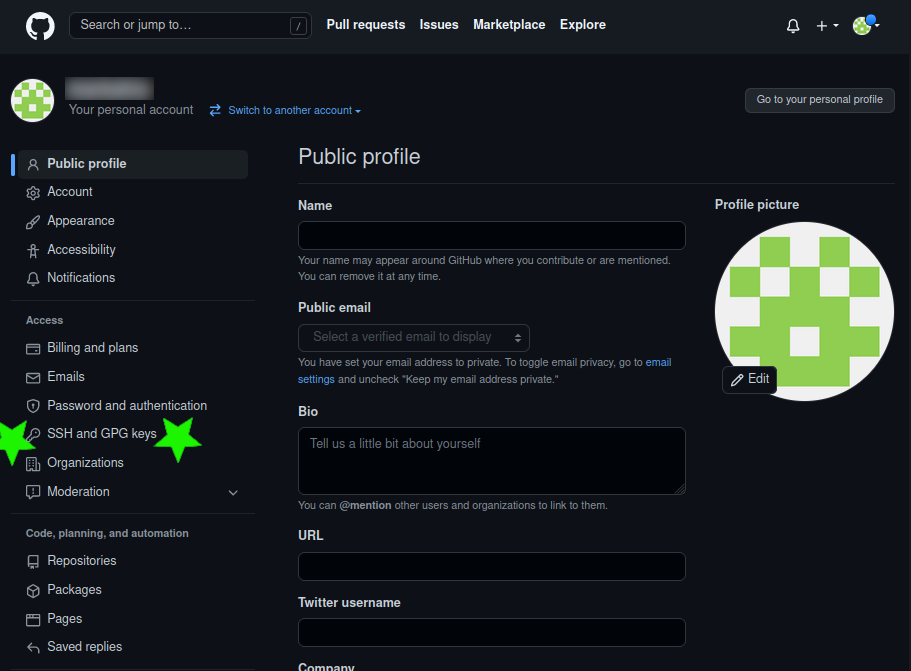
\includegraphics[width=0.8\textwidth]{Images/GH_02.png}
\caption{GitHub Step 2}
\end{figure}
\FloatBarrier

\begin{figure}
\centering
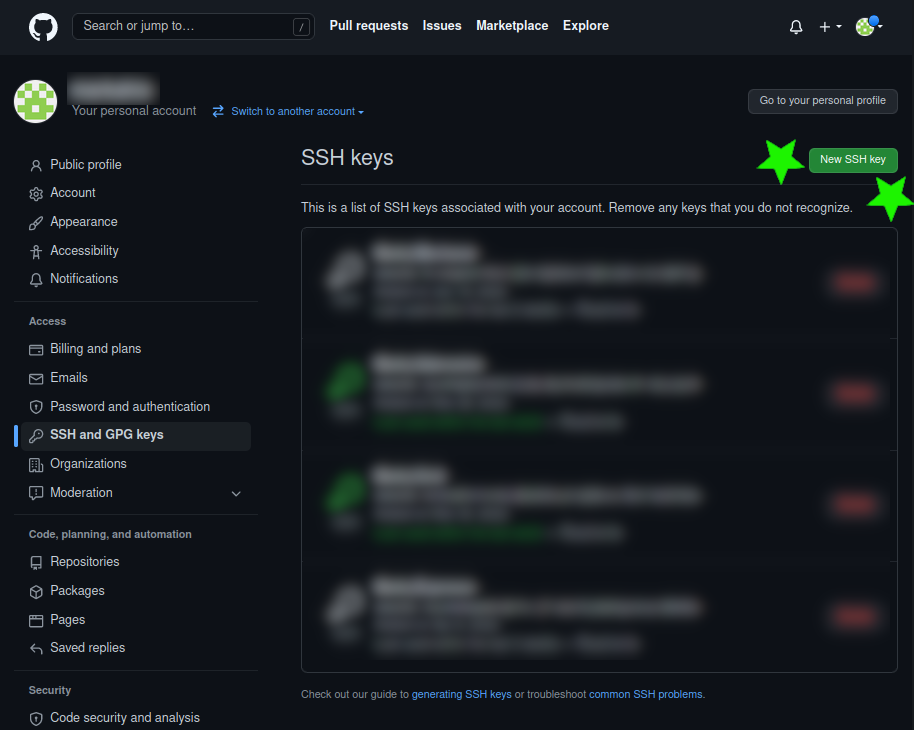
\includegraphics[width=0.8\textwidth]{Images/GH_03.png}
\caption{GitHub Step 3}
\end{figure}
\FloatBarrier

You'll need some text out of a file generated by the \texttt{ssh-keygen}
step. If you named the keyfile \texttt{git\_rsa}, the process will have
also produced a file called \texttt{git\_rsa.pub}, which is the ``public
key'' corresponding to your computer's private key. In simpler terms,
the public key is like a ``secret question'' that the other computer can
ask, that only your computer with its private ``secret answer'' can
properly respond to, so both computers know the other is trusted with
this information transfer.

Open the \texttt{git\_rsa.pub} file and copy all the text into the field
shown on the GitHub website here.

\begin{figure}
\centering
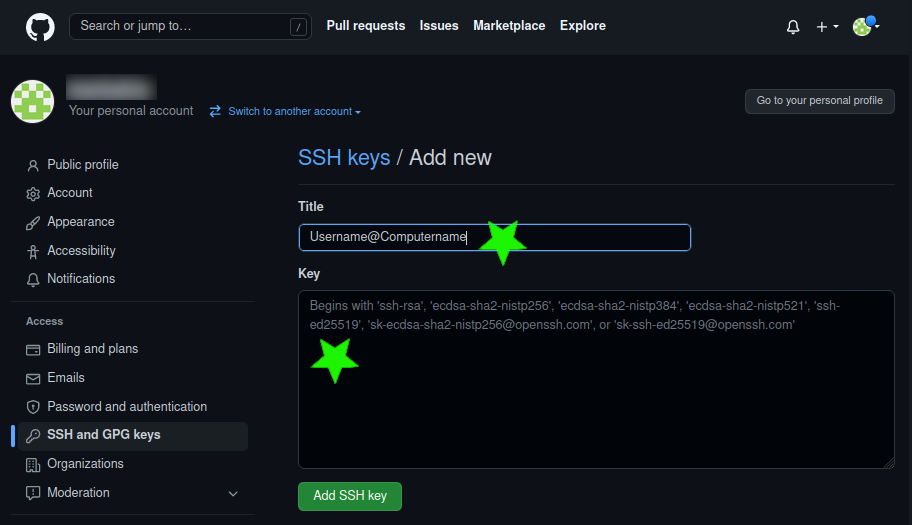
\includegraphics{Images/GH_04.png}
\caption{GitHub Step 4}
\end{figure}
\FloatBarrier

\begin{center}\rule{0.5\linewidth}{0.5pt}\end{center}

You'll also need to configure \texttt{git} on your computer as well.
Assuming you have \texttt{git} already installed, you can begin with
setting some of the initial variables.

You can configure individual repositories (projects) with these
settings, or you can configure \texttt{git} globally to set your
defaults. For now, we'll assume that you only have one GitHub account to
manage on your computer.

\begin{Shaded}
\begin{Highlighting}[]
\FunctionTok{git}\NormalTok{ config }\AttributeTok{{-}{-}global}\NormalTok{ user.name }\StringTok{"Firstname Lastname"}
\FunctionTok{git}\NormalTok{ config }\AttributeTok{{-}{-}global}\NormalTok{ user.email }\StringTok{"username@emailserver.com"}
\FunctionTok{git}\NormalTok{ config }\AttributeTok{{-}{-}global}\NormalTok{ user.user }\StringTok{"github\_username"}
\end{Highlighting}
\end{Shaded}

This next command may not mean too much right now, but it's useful to
have right off the bat to keep things clean later on.

\begin{Shaded}
\begin{Highlighting}[]
\FunctionTok{git}\NormalTok{ config }\AttributeTok{{-}{-}global}\NormalTok{ core.excludesFile }\StringTok{\textquotesingle{}\textasciitilde{}/.gitignore\textquotesingle{}}
\FunctionTok{touch}\NormalTok{ \textasciitilde{}/.gitignore}
\end{Highlighting}
\end{Shaded}

This tells git to ignore anything listed in the file
\texttt{\textasciitilde{}/.gitignore} when maintaining version controls.
This is useful for things like cached files produced by various Python
scripts, compiled programs/object files from C++, and so forth. As we
continue forward, we'll add some things to the global ignore, and others
to repository-specific \texttt{.gitignore} files.

\begin{center}\rule{0.5\linewidth}{0.5pt}\end{center}

Okay, we we've configured \texttt{git} on our computers, now how about
actually \emph{using} it?

Let's say you've made some headway on designing and maybe even coding up
some of your project, and you remember how important it is to maintain
version controls. You can initialize the project folder
\texttt{MyCodingProject} with the following command

\begin{Shaded}
\begin{Highlighting}[]
\FunctionTok{git}\NormalTok{ init MyCodingProject/}
\end{Highlighting}
\end{Shaded}

This establishes a starting point for all future versions to be compared
against.

For more useful commands, check out this cheat sheet!

\begin{figure}
\centering
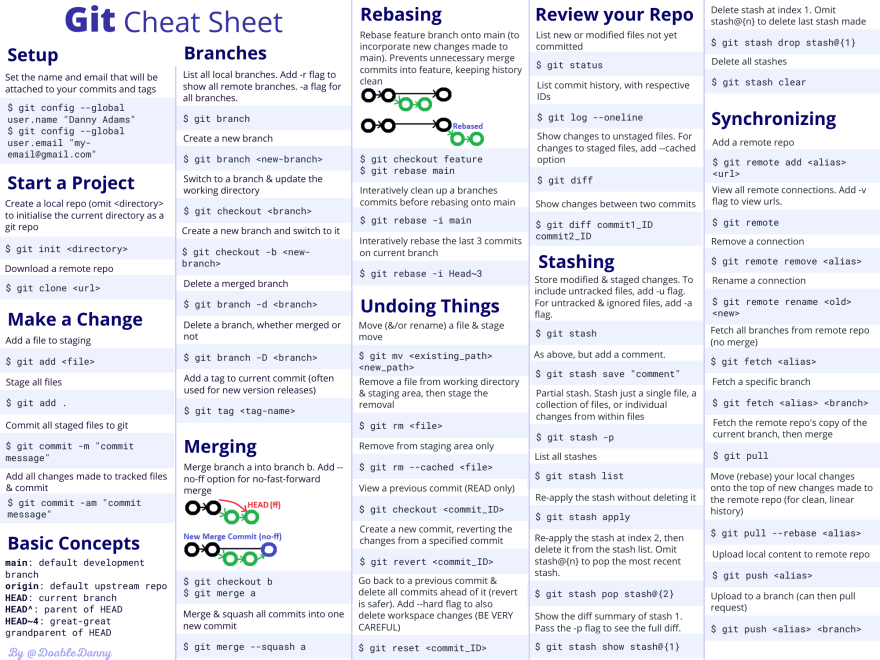
\includegraphics{Images/GitCheatSheet.png}
\caption{Git Cheat Sheet}
\end{figure}
\FloatBarrier

%%%%%%%%%%%%%%%%%%%%%%%%%%%%%%%%%%%%%%%%%%%%%%%%%%%%%%%%%%%%%%%%%%%%%%%%%%%%%%%%%%%%%%%%%%%%%%%%%%%%%%%%%%%%%%%%%%%%%
\section{Code Formatting and Style}
Many different research groups, organizations, and companies have what
are known as ``style guides'' for any code produced in, by, or for the
organization. These often include the simple concepts like ``how many
spaces constitute a \texttt{tab} in your code?'' or ``What information,
if any, should be included in comments at the top of each file?''.
However, these style guides can also include more complex information
beyond text formatting and up into things like ``Each function
definition should include comments describing the arguments to the
function and what the function returns on completion'' or ``Test suites
must be included for all additions to the codebase before they may be
considered for merging''.

Most programming languages have a form of something called
\textbf{scope}, which is a region in the code in which certain things
are true. For example, a function may have variables that only exist
inside that function, and then disappear once the program exits the
function's \textbf{scope}. Some languages use specific characters to
define a scope, such as \texttt{C++} with \texttt{\{} and \texttt{\}}
defining the beginning and end of a scope.

\begin{Shaded}
\begin{Highlighting}[]
\DataTypeTok{int}\NormalTok{ main}\OperatorTok{()}
\OperatorTok{\{}
\NormalTok{    cout }\OperatorTok{\textless{}\textless{}} \StringTok{"Hello World!}\SpecialCharTok{\textbackslash{}n}\StringTok{"}\OperatorTok{;}
    \ControlFlowTok{if} \OperatorTok{(}\DecValTok{5} \OperatorTok{\textless{}} \DecValTok{4}\OperatorTok{)}
    \OperatorTok{\{}
\NormalTok{        cout }\OperatorTok{\textless{}\textless{}} \StringTok{"Five is less than four.}\SpecialCharTok{\textbackslash{}n}\StringTok{"}\OperatorTok{;}
    \OperatorTok{\}}
    \ControlFlowTok{return}\OperatorTok{;}
\OperatorTok{\}}
\end{Highlighting}
\end{Shaded}

A common convention is to use spaces or tabs when moving into different
levels of scope, however this is usually for easier reading by humans
and isn't necessary for the code compiler itself.

Others, like \texttt{Python}, use indentations of spaces or tabs and are
specifically required to change scope.

\begin{Shaded}
\begin{Highlighting}[]
\KeywordTok{def}\NormalTok{ myfunction(x):}
\NormalTok{    x }\OperatorTok{=}\NormalTok{ x }\OperatorTok{+} \DecValTok{5}
    \BuiltInTok{print}\NormalTok{(x)}
    \ControlFlowTok{return}

\NormalTok{x }\OperatorTok{=} \DecValTok{10}
\BuiltInTok{print}\NormalTok{(x)}
\NormalTok{myfunction(x)}
\BuiltInTok{print}\NormalTok{(x)}
\end{Highlighting}
\end{Shaded}

The code snippet above shows the variable x inside the scope of
\texttt{myfunction} as well as the main program. If we follow the value
of \texttt{x} as the program runs, we can see that \texttt{x\ =\ 10},
which is printed out. Then, the \emph{value} of \texttt{x} is passed
into the function, which adds five and prints it out
(\texttt{x\ =\ 15}). Once that is done, the function returns, and the
main program's value of x is printed out again. (\texttt{x\ =\ 10}).

Let's see how that works in practice.

    \begin{tcolorbox}[breakable, size=fbox, boxrule=1pt, pad at break*=1mm,colback=cellbackground, colframe=cellborder]
\prompt{In}{incolor}{2}{\boxspacing}
\begin{Verbatim}[commandchars=\\\{\}]
\PY{k}{def} \PY{n+nf}{myfunction}\PY{p}{(}\PY{n}{x}\PY{p}{)}\PY{p}{:}
    \PY{n}{x} \PY{o}{=} \PY{n}{x} \PY{o}{+} \PY{l+m+mi}{5}
    \PY{n+nb}{print}\PY{p}{(}\PY{n}{x}\PY{p}{)}
    \PY{k}{return}

\PY{n}{x} \PY{o}{=} \PY{l+m+mi}{10}
\PY{n+nb}{print}\PY{p}{(}\PY{n}{x}\PY{p}{)}
\PY{n}{myfunction}\PY{p}{(}\PY{n}{x}\PY{p}{)}
\PY{n+nb}{print}\PY{p}{(}\PY{n}{x}\PY{p}{)}
\end{Verbatim}
\end{tcolorbox}

    \begin{Verbatim}[commandchars=\\\{\}]
10
15
10
    \end{Verbatim}

    It is very important to keep scope in mind when using variables as
counters or other housekeepers.

Many programmers use \texttt{i} as a counter variable in loops. However,
sometimes it is necessary to have loops inside other loops (nested),
which effectively means you have a scope inside another scope. If you
use \texttt{i} in the outer loop, then change it in the inner loop, it
remains changed in the outer loop and can have effects on the execution
of your code.

Therefore, it is important to keep track of what variables are used
during the execution of your code and how they are modified as you go.

\hypertarget{back-to-formatting}{%
\paragraph{Back to Formatting}\label{back-to-formatting}}

Formatting is not simply a matter of using indents or
80-characters-per-line requirements. Formatting also includes things
like expected code-comments or other internal documentation. Some code
development packages have the functionality built in to parse comments
in the code and build human-readable documentation, but it requires the
use of specific formats in the comments. See the examples below.

    \begin{tcolorbox}[breakable, size=fbox, boxrule=1pt, pad at break*=1mm,colback=cellbackground, colframe=cellborder]
\prompt{In}{incolor}{3}{\boxspacing}
\begin{Verbatim}[commandchars=\\\{\}]
\PY{k+kn}{import} \PY{n+nn}{numpy} \PY{k}{as} \PY{n+nn}{np}
\PY{k}{def} \PY{n+nf}{myfunction}\PY{p}{(}\PY{n}{x}\PY{p}{,}\PY{n}{y}\PY{p}{,}\PY{n}{z}\PY{p}{)}\PY{p}{:}
    \PY{n}{norm} \PY{o}{=} \PY{n}{np}\PY{o}{.}\PY{n}{linalg}\PY{o}{.}\PY{n}{norm}\PY{p}{(}\PY{p}{[}\PY{n}{x}\PY{p}{,}\PY{n}{y}\PY{p}{,}\PY{n}{z}\PY{p}{]}\PY{p}{)}
    \PY{k}{return} \PY{n}{norm}
\PY{n}{a} \PY{o}{=} \PY{l+m+mi}{1}
\PY{n}{b} \PY{o}{=} \PY{l+m+mi}{2}
\PY{n}{c} \PY{o}{=} \PY{l+m+mi}{3}
\PY{n}{result} \PY{o}{=} \PY{n}{myfunction}\PY{p}{(}\PY{n}{a}\PY{p}{,}\PY{n}{b}\PY{p}{,}\PY{n}{c}\PY{p}{)}
\PY{n+nb}{print}\PY{p}{(}\PY{n}{result}\PY{p}{)}
\end{Verbatim}
\end{tcolorbox}

    \begin{Verbatim}[commandchars=\\\{\}]
3.7416573867739413
    \end{Verbatim}

    The code block above has no comments in it, and so without already
knowing what the individual parts are doing, it's not easy to know what
is happening in the code or how to modify and manipulate it for your own
purposes. If we take the same code block and add some commentary, it can
be made easier.

    \begin{tcolorbox}[breakable, size=fbox, boxrule=1pt, pad at break*=1mm,colback=cellbackground, colframe=cellborder]
\prompt{In}{incolor}{4}{\boxspacing}
\begin{Verbatim}[commandchars=\\\{\}]
\PY{c+c1}{\PYZsh{} library import}
\PY{k+kn}{import} \PY{n+nn}{numpy} \PY{k}{as} \PY{n+nn}{np}

\PY{c+c1}{\PYZsh{} function definition}
\PY{k}{def} \PY{n+nf}{myfunction}\PY{p}{(}\PY{n}{x}\PY{p}{,}\PY{n}{y}\PY{p}{,}\PY{n}{z}\PY{p}{)}\PY{p}{:}
    \PY{n}{norm} \PY{o}{=} \PY{n}{np}\PY{o}{.}\PY{n}{linalg}\PY{o}{.}\PY{n}{norm}\PY{p}{(}\PY{p}{[}\PY{n}{x}\PY{p}{,}\PY{n}{y}\PY{p}{,}\PY{n}{z}\PY{p}{]}\PY{p}{)}
    \PY{k}{return} \PY{n}{norm}

\PY{c+c1}{\PYZsh{} Main program execution}
\PY{n}{a} \PY{o}{=} \PY{l+m+mi}{1}
\PY{n}{b} \PY{o}{=} \PY{l+m+mi}{2}
\PY{n}{c} \PY{o}{=} \PY{l+m+mi}{3}
\PY{n}{result} \PY{o}{=} \PY{n}{myfunction}\PY{p}{(}\PY{n}{a}\PY{p}{,}\PY{n}{b}\PY{p}{,}\PY{n}{c}\PY{p}{)}
\PY{n+nb}{print}\PY{p}{(}\PY{n}{result}\PY{p}{)}
\end{Verbatim}
\end{tcolorbox}

    \begin{Verbatim}[commandchars=\\\{\}]
3.7416573867739413
    \end{Verbatim}

    Now we have a little more clarity in what is happening, but it can still
be made clearer. As it stands, we simply know that we're importing
libraries, defining a function, and running the main program.

We can improve the commentary further by describing what is happening in
the function or the steps inside the main program.

    \begin{tcolorbox}[breakable, size=fbox, boxrule=1pt, pad at break*=1mm,colback=cellbackground, colframe=cellborder]
\prompt{In}{incolor}{5}{\boxspacing}
\begin{Verbatim}[commandchars=\\\{\}]
\PY{c+c1}{\PYZsh{} library import}
\PY{k+kn}{import} \PY{n+nn}{numpy} \PY{k}{as} \PY{n+nn}{np}

\PY{c+c1}{\PYZsh{} function definition}
\PY{k}{def} \PY{n+nf}{myfunction}\PY{p}{(}\PY{n}{x}\PY{p}{,}\PY{n}{y}\PY{p}{,}\PY{n}{z}\PY{p}{)}\PY{p}{:}
    \PY{c+c1}{\PYZsh{} Arguments:}
    \PY{c+c1}{\PYZsh{} x \PYZhy{} float representing the x component of a vector}
    \PY{c+c1}{\PYZsh{} y \PYZhy{} float representing the y component of a vector}
    \PY{c+c1}{\PYZsh{} z \PYZhy{} float representing the z component of a vector}
    \PY{c+c1}{\PYZsh{} Returns:}
    \PY{c+c1}{\PYZsh{} norm \PYZhy{} float representing the magnitude of the vector given by the [x,y,z] values}
    \PY{n}{norm} \PY{o}{=} \PY{n}{np}\PY{o}{.}\PY{n}{linalg}\PY{o}{.}\PY{n}{norm}\PY{p}{(}\PY{p}{[}\PY{n}{x}\PY{p}{,}\PY{n}{y}\PY{p}{,}\PY{n}{z}\PY{p}{]}\PY{p}{)}
    \PY{k}{return} \PY{n}{norm}

\PY{c+c1}{\PYZsh{} Main program execution}
\PY{c+c1}{\PYZsh{} initialize variables }
\PY{n}{a} \PY{o}{=} \PY{l+m+mi}{1}
\PY{n}{b} \PY{o}{=} \PY{l+m+mi}{2}
\PY{n}{c} \PY{o}{=} \PY{l+m+mi}{3}
\PY{c+c1}{\PYZsh{} obtain the magnitude of the vector defined by [a,b,c]}
\PY{n}{result} \PY{o}{=} \PY{n}{myfunction}\PY{p}{(}\PY{n}{a}\PY{p}{,}\PY{n}{b}\PY{p}{,}\PY{n}{c}\PY{p}{)}
\PY{c+c1}{\PYZsh{} print out the magnitude}
\PY{n+nb}{print}\PY{p}{(}\PY{n}{result}\PY{p}{)}
\end{Verbatim}
\end{tcolorbox}

    \begin{Verbatim}[commandchars=\\\{\}]
3.7416573867739413
    \end{Verbatim}

    With this level of commentary in the code, we can easily understand what
is happening in the function and the main code block. This is very
useful when working on collaborative projects especially, as it can
ensure that everyone is able to follow your thought process in the code
and, if necessary, compare to the actual code for debugging purposes.

Another thing to consider is the larger format of a project. That is,
not simply how the text is arranged in a file, but how code blocks and
functions are arranged in multiple files. For smaller programs, it may
not be necessary to divide the code up in this way, but for larger
projects - or for standard functions you'll use in multiple separate
projects - it may be easier and cleaner to keep some things separated
and compartmentalized. This also makes compiling easier later on down
the line.

It can also lead to smaller individual files, making debugging easier as
well - most error messages include the location where the error was
encountered, and it's much easier to go to
\texttt{line\ 46\ in\ utility.cpp} than it is to go to
\texttt{line\ 57684\ in\ main.cpp}. As a bonus, making changes in
smaller files won't necessarily require the entire codebase to be
recompiled, but rather just the small portion you modified.



\chapter{Thinking Like a Computer}
%%%%%%%%%%%%%%%%%%%%%%%%%%%%%%%%%%%%%%%%%%%%%%%%%%%%%%%%%%%%%%%%%%%%%%%%%%%%%%%%%%%%%%%%%%%%%%%%%%%%%%%%%%%%%%%%%%%%%
\section{Pseudocode}
Other names for pseudocode include ``algorithm development'', ``project management'', ``outlining'', ``planning'', ``thinking'', and ``jotting that down so I don't forget it later''.
Pseudocoding is effectively just writing out the stages of your program in plain language (\emph{not code}) to ensure a clear understanding of the problem you're trying to solve. 
Often, programmers will begin pseudocode with a very simple set of steps they think of the problem. 
Each step can be explained in more and more detail as a set of smaller, more manageable steps, until eventually you wind up with a complete list of steps that can be converted to computer commands. 
Pseudocode can also provide some insight into ways the code might be optimized, such as by revealing opportunities to parallelise the execution, or by revealing regions where something being calculated can just be saved for reuse rather than recalculated again later.

One of the most valuable skills a programmer can develop is the ability to think like a computer.
This means learning to break down larger problems and complex behaviors into smaller and smaller pieces until it becomes a collection of tiny calculations such as a sequence of additions and subtractions, or comparisons between two values.

A good habit to develop whenever beginning a new project is to first outline the expected flow of the code. 
Some people use a whiteboard, or scratch paper, or just a blank text document on their computer - it doesn't matter how you do it, just that you plan it out somehow before jumping into the code.

\hypertarget{example-project---brownian-motion}{%
\paragraph{Example Project - Brownian
Motion}\label{example-project---brownian-motion}}

Write a program that places an arbitrary number of particles in a box of
some other arbitrary size, then moves them around randomly by assigning
a random x, y, and z component of their motion vector between 0 and 1.

Remember to just write in pseudocode. 
You can make it as complex as you like, but
it should just be plain text. Try to think through the steps of the
problem like a computer might.

% Once you've completed your pseudocode, keep it handy - you can use it
% for tomorrow's project!

\section{Data and Variable Types}
Different types of information can be stored for use by the computer. 
Some programming languages are fairly lenient about variable types and are flexible with what types of data are being provided in a given variable. 
Others are a bit more strict, and require explicit type declarations/definitions for each variable to ensure proper memory allocation. 
\emph{If only some of that made sense, you're in the right place.}

C++ requires that every variable have a clearly defined type, which the compiler uses to ensure the program allocates the correct amount of memory at runtime.
Python doesn't generally require \emph{explicit} variable type declarations (with some exceptions that will come later as we get into more advanced programming). 
However, it is still useful to know what kinds of data there is, what can be done with it, and how it's stored.

First, let's explore data types like \texttt{int}, \texttt{float},
\texttt{list}, \texttt{tuple}, and \texttt{string}.

    \begin{tcolorbox}[breakable, size=fbox, boxrule=1pt, pad at break*=1mm,colback=cellbackground, colframe=cellborder]
\prompt{In}{incolor}{1}{\boxspacing}
\begin{Verbatim}[commandchars=\\\{\}]
\PY{n}{my\PYZus{}int}    \PY{o}{=} \PY{l+m+mi}{2}
\PY{n}{my\PYZus{}float}  \PY{o}{=} \PY{l+m+mf}{3.1415}
\PY{n}{my\PYZus{}list}   \PY{o}{=} \PY{p}{[}\PY{l+m+mi}{1}\PY{p}{,}\PY{l+m+mf}{3.1415}\PY{p}{,}\PY{l+s+s2}{\PYZdq{}}\PY{l+s+s2}{Hello World!}\PY{l+s+s2}{\PYZdq{}}\PY{p}{,}\PY{l+s+s2}{\PYZdq{}}\PY{l+s+s2}{pizza}\PY{l+s+s2}{\PYZdq{}}\PY{p}{]}
\PY{n}{my\PYZus{}tuple}  \PY{o}{=} \PY{p}{(}\PY{l+m+mi}{5}\PY{p}{,}\PY{l+m+mi}{6}\PY{p}{,}\PY{l+m+mi}{7}\PY{p}{,}\PY{l+m+mi}{8}\PY{p}{,}\PY{l+m+mi}{9}\PY{p}{)}
\PY{n}{my\PYZus{}string} \PY{o}{=} \PY{l+s+s2}{\PYZdq{}}\PY{l+s+s2}{Hello World!}\PY{l+s+s2}{\PYZdq{}}
\end{Verbatim}
\end{tcolorbox}

    These examples are fairly simple.

\begin{itemize}
\tightlist
\item
  \texttt{my\_int} is an integer, and gets treated like one. Integers
  are useful for things like indexes, counters, and so forth.
\item
  \texttt{my\_float} is a float (often called a ``double'' in other
  programming languages), and are regular numbers including decimals.
\item
  \texttt{my\_list} is a list of values enclosed in square brackets.
  Lists are indexed from zero, which means the first item in a list is
  ``item 0''. Lists are great ways to keep collections of data organized
  and in order, and you can extract individual values simply by
  including the index with the variable name: \texttt{my\_list{[}3{]}}
  will return ``pizza''. You can also get values from the end of a list
  with negative indices. my\_list\texttt{{[}-1{]}} will return ``pizza''
  because it's the last value.
\item
  \texttt{my\_tuple} is similar to a list, except that it is a little
  more difficult to pull individual values from it. Tuples are useful
  when you need to maintain groups of values together in relation to
  each other, such as with (x,y,z) coordinates.
\item
  \texttt{my\_string} is a list of characters including letters,
  numbers, punctuation, whitespace (tabs, spaces, line breaks, etc.).
  The contents of a string do not include the quotation marks on either
  side. Strings can include quotes using \emph{escapes} like
  \texttt{\textbackslash{}"} or
  \texttt{\textbackslash{}\textbackslash{}} to include a backslash.
\end{itemize}

Variable manipulation comes in many forms and depends on the type of
data contained within. Better understanding of how data types work can
allow you to do some interesting things, like taking a ``slice'' of a
string like you would from a list.

Consider the examples below.

    \begin{tcolorbox}[breakable, size=fbox, boxrule=1pt, pad at break*=1mm,colback=cellbackground, colframe=cellborder]
\prompt{In}{incolor}{2}{\boxspacing}
\begin{Verbatim}[commandchars=\\\{\}]
\PY{n}{my\PYZus{}list} \PY{o}{=} \PY{p}{[}\PY{l+m+mi}{0}\PY{p}{,}\PY{l+m+mi}{1}\PY{p}{,}\PY{l+m+mi}{2}\PY{p}{,}\PY{l+m+mi}{3}\PY{p}{,}\PY{l+m+mi}{4}\PY{p}{,}\PY{l+m+mi}{5}\PY{p}{,}\PY{l+m+mi}{6}\PY{p}{,}\PY{l+m+mi}{7}\PY{p}{,}\PY{l+m+mi}{8}\PY{p}{,}\PY{l+m+mi}{9}\PY{p}{,}\PY{l+m+mi}{10}\PY{p}{,}\PY{l+m+mi}{11}\PY{p}{,}\PY{l+m+mi}{12}\PY{p}{,}\PY{l+m+mi}{13}\PY{p}{,}\PY{l+m+mi}{14}\PY{p}{,}\PY{l+m+mi}{15}\PY{p}{,}\PY{l+m+mi}{16}\PY{p}{,}\PY{l+m+mi}{17}\PY{p}{,}\PY{l+m+mi}{18}\PY{p}{,}\PY{l+m+mi}{19}\PY{p}{,}\PY{l+m+mi}{20}\PY{p}{,}\PY{l+m+mi}{21}\PY{p}{,}\PY{l+m+mi}{22}\PY{p}{,}\PY{l+m+mi}{23}\PY{p}{,}\PY{l+m+mi}{24}\PY{p}{,}\PY{l+m+mi}{25}\PY{p}{]}
\PY{c+c1}{\PYZsh{} my\PYZus{}list has a length of 26 individual values}
\PY{n+nb}{len}\PY{p}{(}\PY{n}{my\PYZus{}list}\PY{p}{)}
\end{Verbatim}
\end{tcolorbox}

            \begin{tcolorbox}[breakable, size=fbox, boxrule=.5pt, pad at break*=1mm, opacityfill=0]
\prompt{Out}{outcolor}{2}{\boxspacing}
\begin{Verbatim}[commandchars=\\\{\}]
26
\end{Verbatim}
\end{tcolorbox}
        
    \begin{tcolorbox}[breakable, size=fbox, boxrule=1pt, pad at break*=1mm,colback=cellbackground, colframe=cellborder]
\prompt{In}{incolor}{3}{\boxspacing}
\begin{Verbatim}[commandchars=\\\{\}]
\PY{n}{my\PYZus{}string} \PY{o}{=} \PY{l+s+s2}{\PYZdq{}}\PY{l+s+s2}{Once more into the breach!}\PY{l+s+s2}{\PYZdq{}}
\PY{c+c1}{\PYZsh{} my\PYZus{}string has a length of 26 characters including whitespace and punctuation.}
\PY{n+nb}{len}\PY{p}{(}\PY{n}{my\PYZus{}string}\PY{p}{)}
\end{Verbatim}
\end{tcolorbox}

            \begin{tcolorbox}[breakable, size=fbox, boxrule=.5pt, pad at break*=1mm, opacityfill=0]
\prompt{Out}{outcolor}{3}{\boxspacing}
\begin{Verbatim}[commandchars=\\\{\}]
26
\end{Verbatim}
\end{tcolorbox}
        
    \hypertarget{slicing-lists}{%
\subsubsection{Slicing Lists}\label{slicing-lists}}

One common use for lists is ``slicing'', where you can get a small
subsection of the list. Let's say you wanted just the first five
elements in \texttt{my\_list}. You would use a slice. Slices are
generated similar to how an individual element is called from a list,
from inside square brackets. However, we can put a \texttt{:} between
the starting and ending indices to get everything between. We can also
use an empty space to indicate ``everything''. Check out the examples
below.

    \begin{tcolorbox}[breakable, size=fbox, boxrule=1pt, pad at break*=1mm,colback=cellbackground, colframe=cellborder]
\prompt{In}{incolor}{4}{\boxspacing}
\begin{Verbatim}[commandchars=\\\{\}]
\PY{n}{my\PYZus{}list}\PY{p}{[}\PY{p}{:}\PY{l+m+mi}{5}\PY{p}{]}
\end{Verbatim}
\end{tcolorbox}

            \begin{tcolorbox}[breakable, size=fbox, boxrule=.5pt, pad at break*=1mm, opacityfill=0]
\prompt{Out}{outcolor}{4}{\boxspacing}
\begin{Verbatim}[commandchars=\\\{\}]
[0, 1, 2, 3, 4]
\end{Verbatim}
\end{tcolorbox}
        
    \begin{tcolorbox}[breakable, size=fbox, boxrule=1pt, pad at break*=1mm,colback=cellbackground, colframe=cellborder]
\prompt{In}{incolor}{5}{\boxspacing}
\begin{Verbatim}[commandchars=\\\{\}]
\PY{n}{my\PYZus{}list}\PY{p}{[}\PY{l+m+mi}{5}\PY{p}{:}\PY{l+m+mi}{10}\PY{p}{]}
\end{Verbatim}
\end{tcolorbox}

            \begin{tcolorbox}[breakable, size=fbox, boxrule=.5pt, pad at break*=1mm, opacityfill=0]
\prompt{Out}{outcolor}{5}{\boxspacing}
\begin{Verbatim}[commandchars=\\\{\}]
[5, 6, 7, 8, 9]
\end{Verbatim}
\end{tcolorbox}
        
    Note how the two results are different. The ending in the first cell is
the same as the beginning of the second cell, but we don't actually get
``5'' in the results in the first cell. Slices go ``up to'' the ending
value, but don't include it. Keep this in mind when working with slices.
We can also combine other tricks from list manipulations, like using
negative indices to go backwards from the end.

In the next cell, we'll get the last seven elements from the list.

    \begin{tcolorbox}[breakable, size=fbox, boxrule=1pt, pad at break*=1mm,colback=cellbackground, colframe=cellborder]
\prompt{In}{incolor}{6}{\boxspacing}
\begin{Verbatim}[commandchars=\\\{\}]
\PY{n}{my\PYZus{}list}\PY{p}{[}\PY{o}{\PYZhy{}}\PY{l+m+mi}{7}\PY{p}{:}\PY{p}{]}
\end{Verbatim}
\end{tcolorbox}

            \begin{tcolorbox}[breakable, size=fbox, boxrule=.5pt, pad at break*=1mm, opacityfill=0]
\prompt{Out}{outcolor}{6}{\boxspacing}
\begin{Verbatim}[commandchars=\\\{\}]
[19, 20, 21, 22, 23, 24, 25]
\end{Verbatim}
\end{tcolorbox}
        
    What if we wanted every third element in the list?

    \begin{tcolorbox}[breakable, size=fbox, boxrule=1pt, pad at break*=1mm,colback=cellbackground, colframe=cellborder]
\prompt{In}{incolor}{7}{\boxspacing}
\begin{Verbatim}[commandchars=\\\{\}]
\PY{n}{my\PYZus{}list}\PY{p}{[}\PY{p}{:}\PY{p}{:}\PY{l+m+mi}{3}\PY{p}{]}
\end{Verbatim}
\end{tcolorbox}

            \begin{tcolorbox}[breakable, size=fbox, boxrule=.5pt, pad at break*=1mm, opacityfill=0]
\prompt{Out}{outcolor}{7}{\boxspacing}
\begin{Verbatim}[commandchars=\\\{\}]
[0, 3, 6, 9, 12, 15, 18, 21, 24]
\end{Verbatim}
\end{tcolorbox}
        
    The second \texttt{:} indicates a ``stride''. This is useful when you
have data that is strangely shaped (such as a long list of values that
correspond to x,y,z coordinates, but aren't in a (3,n) shaped list.

Now let's combine these. We'll get every other element starting from the
tenth and going up to the twentieth.

    \begin{tcolorbox}[breakable, size=fbox, boxrule=1pt, pad at break*=1mm,colback=cellbackground, colframe=cellborder]
\prompt{In}{incolor}{8}{\boxspacing}
\begin{Verbatim}[commandchars=\\\{\}]
\PY{n}{my\PYZus{}list}\PY{p}{[}\PY{l+m+mi}{10}\PY{p}{:}\PY{l+m+mi}{20}\PY{p}{:}\PY{l+m+mi}{2}\PY{p}{]}
\end{Verbatim}
\end{tcolorbox}

            \begin{tcolorbox}[breakable, size=fbox, boxrule=.5pt, pad at break*=1mm, opacityfill=0]
\prompt{Out}{outcolor}{8}{\boxspacing}
\begin{Verbatim}[commandchars=\\\{\}]
[10, 12, 14, 16, 18]
\end{Verbatim}
\end{tcolorbox}
        
    Now let's look at strings. Strings are just lists of letters, numbers,
and any other characters you can think of. With this in mind, we can do
things to strings that we have done to lists.

    \begin{tcolorbox}[breakable, size=fbox, boxrule=1pt, pad at break*=1mm,colback=cellbackground, colframe=cellborder]
\prompt{In}{incolor}{9}{\boxspacing}
\begin{Verbatim}[commandchars=\\\{\}]
\PY{n}{my\PYZus{}string}
\end{Verbatim}
\end{tcolorbox}

            \begin{tcolorbox}[breakable, size=fbox, boxrule=.5pt, pad at break*=1mm, opacityfill=0]
\prompt{Out}{outcolor}{9}{\boxspacing}
\begin{Verbatim}[commandchars=\\\{\}]
'Once more into the breach!'
\end{Verbatim}
\end{tcolorbox}
        
    \begin{tcolorbox}[breakable, size=fbox, boxrule=1pt, pad at break*=1mm,colback=cellbackground, colframe=cellborder]
\prompt{In}{incolor}{10}{\boxspacing}
\begin{Verbatim}[commandchars=\\\{\}]
\PY{n}{my\PYZus{}string}\PY{p}{[}\PY{p}{:}\PY{l+m+mi}{5}\PY{p}{]}
\end{Verbatim}
\end{tcolorbox}

            \begin{tcolorbox}[breakable, size=fbox, boxrule=.5pt, pad at break*=1mm, opacityfill=0]
\prompt{Out}{outcolor}{10}{\boxspacing}
\begin{Verbatim}[commandchars=\\\{\}]
'Once '
\end{Verbatim}
\end{tcolorbox}
        
    \begin{tcolorbox}[breakable, size=fbox, boxrule=1pt, pad at break*=1mm,colback=cellbackground, colframe=cellborder]
\prompt{In}{incolor}{11}{\boxspacing}
\begin{Verbatim}[commandchars=\\\{\}]
\PY{n}{my\PYZus{}string}\PY{p}{[}\PY{l+m+mi}{5}\PY{p}{:}\PY{l+m+mi}{10}\PY{p}{]}
\end{Verbatim}
\end{tcolorbox}

            \begin{tcolorbox}[breakable, size=fbox, boxrule=.5pt, pad at break*=1mm, opacityfill=0]
\prompt{Out}{outcolor}{11}{\boxspacing}
\begin{Verbatim}[commandchars=\\\{\}]
'more '
\end{Verbatim}
\end{tcolorbox}
        
    \begin{tcolorbox}[breakable, size=fbox, boxrule=1pt, pad at break*=1mm,colback=cellbackground, colframe=cellborder]
\prompt{In}{incolor}{12}{\boxspacing}
\begin{Verbatim}[commandchars=\\\{\}]
\PY{n}{my\PYZus{}string}\PY{p}{[}\PY{o}{\PYZhy{}}\PY{l+m+mi}{7}\PY{p}{:}\PY{p}{]}
\end{Verbatim}
\end{tcolorbox}

            \begin{tcolorbox}[breakable, size=fbox, boxrule=.5pt, pad at break*=1mm, opacityfill=0]
\prompt{Out}{outcolor}{12}{\boxspacing}
\begin{Verbatim}[commandchars=\\\{\}]
'breach!'
\end{Verbatim}
\end{tcolorbox}
        
    \begin{tcolorbox}[breakable, size=fbox, boxrule=1pt, pad at break*=1mm,colback=cellbackground, colframe=cellborder]
\prompt{In}{incolor}{13}{\boxspacing}
\begin{Verbatim}[commandchars=\\\{\}]
\PY{n}{my\PYZus{}string}\PY{p}{[}\PY{p}{:}\PY{p}{:}\PY{l+m+mi}{3}\PY{p}{]}
\end{Verbatim}
\end{tcolorbox}

            \begin{tcolorbox}[breakable, size=fbox, boxrule=.5pt, pad at break*=1mm, opacityfill=0]
\prompt{Out}{outcolor}{13}{\boxspacing}
\begin{Verbatim}[commandchars=\\\{\}]
'Oeo tt eh'
\end{Verbatim}
\end{tcolorbox}
        
    \begin{tcolorbox}[breakable, size=fbox, boxrule=1pt, pad at break*=1mm,colback=cellbackground, colframe=cellborder]
\prompt{In}{incolor}{14}{\boxspacing}
\begin{Verbatim}[commandchars=\\\{\}]
\PY{n}{my\PYZus{}string}\PY{p}{[}\PY{l+m+mi}{10}\PY{p}{:}\PY{l+m+mi}{20}\PY{p}{:}\PY{l+m+mi}{2}\PY{p}{]}
\end{Verbatim}
\end{tcolorbox}

            \begin{tcolorbox}[breakable, size=fbox, boxrule=.5pt, pad at break*=1mm, opacityfill=0]
\prompt{Out}{outcolor}{14}{\boxspacing}
\begin{Verbatim}[commandchars=\\\{\}]
'it h '
\end{Verbatim}
\end{tcolorbox}
        
    \ldots{} some functions are more useful than others, but you get the
idea!

Now let's look at integers and floats. In some programming languages,
the difference between these two can be pretty severe. For example, in
C++, dividing a double by an integer will give you a truncated integer,
which means you can lose some of the information in your data if you're
not careful. Thankfully, Python is a little more forgiving.

Normal division works like we might intuitively expect, where a float
divided by an integer can be a float, and is therefore assumed to be.

    \begin{tcolorbox}[breakable, size=fbox, boxrule=1pt, pad at break*=1mm,colback=cellbackground, colframe=cellborder]
\prompt{In}{incolor}{15}{\boxspacing}
\begin{Verbatim}[commandchars=\\\{\}]
\PY{n}{my\PYZus{}float}\PY{o}{/}\PY{n}{my\PYZus{}int}
\end{Verbatim}
\end{tcolorbox}

            \begin{tcolorbox}[breakable, size=fbox, boxrule=.5pt, pad at break*=1mm, opacityfill=0]
\prompt{Out}{outcolor}{15}{\boxspacing}
\begin{Verbatim}[commandchars=\\\{\}]
1.57075
\end{Verbatim}
\end{tcolorbox}
        
    We can also force the division to return an integer value (which is
useful in some situations)

In the example above, we got a value of 1.57075. If we were to round
this using conventional methods, we'd get 2 However, forcing integer
division with the \texttt{//} below gives us a truncated (not rounded)
value of 1.0. This is also slightly deceptive, as the \texttt{.0}
implies the value is a float,even though the result is a whole number.
This is important to be aware of when doing mathematical work in python.
Truncation just removes everything after the decimal point, while
rounding actually considers the value beforehand.

    \begin{tcolorbox}[breakable, size=fbox, boxrule=1pt, pad at break*=1mm,colback=cellbackground, colframe=cellborder]
\prompt{In}{incolor}{16}{\boxspacing}
\begin{Verbatim}[commandchars=\\\{\}]
\PY{n}{my\PYZus{}float}\PY{o}{/}\PY{o}{/}\PY{n}{my\PYZus{}int}
\end{Verbatim}
\end{tcolorbox}

            \begin{tcolorbox}[breakable, size=fbox, boxrule=.5pt, pad at break*=1mm, opacityfill=0]
\prompt{Out}{outcolor}{16}{\boxspacing}
\begin{Verbatim}[commandchars=\\\{\}]
1.0
\end{Verbatim}
\end{tcolorbox}
        
    \begin{tcolorbox}[breakable, size=fbox, boxrule=1pt, pad at break*=1mm,colback=cellbackground, colframe=cellborder]
\prompt{In}{incolor}{17}{\boxspacing}
\begin{Verbatim}[commandchars=\\\{\}]
\PY{n+nb}{round}\PY{p}{(}\PY{n}{my\PYZus{}float}\PY{o}{/}\PY{n}{my\PYZus{}int}\PY{p}{)}
\end{Verbatim}
\end{tcolorbox}

            \begin{tcolorbox}[breakable, size=fbox, boxrule=.5pt, pad at break*=1mm, opacityfill=0]
\prompt{Out}{outcolor}{17}{\boxspacing}
\begin{Verbatim}[commandchars=\\\{\}]
2
\end{Verbatim}
\end{tcolorbox}
        
    \hypertarget{math-with-variables}{%
\subsubsection{Math with Variables}\label{math-with-variables}}

Math can get incredibly complex, so it's important to remember your
Order of Operations (PEMDAS) - Parentheses, Exponents, Multiplication,
Division, Addition, and Subtraction.

However, in python it's a little different. Parentheses are solved
first, then exponents, until everything in a given equation is reduced
down to a series of terms separated by \texttt{+},\texttt{-},\texttt{*},
and \texttt{/}. Then, the values are processed left-to-right.

    \begin{tcolorbox}[breakable, size=fbox, boxrule=1pt, pad at break*=1mm,colback=cellbackground, colframe=cellborder]
\prompt{In}{incolor}{18}{\boxspacing}
\begin{Verbatim}[commandchars=\\\{\}]
\PY{l+m+mi}{1} \PY{o}{+} \PY{l+m+mi}{2} \PY{o}{\PYZhy{}} \PY{l+m+mi}{3} \PY{o}{*} \PY{l+m+mi}{4} \PY{o}{/} \PY{l+m+mi}{5}
\end{Verbatim}
\end{tcolorbox}

            \begin{tcolorbox}[breakable, size=fbox, boxrule=.5pt, pad at break*=1mm, opacityfill=0]
\prompt{Out}{outcolor}{18}{\boxspacing}
\begin{Verbatim}[commandchars=\\\{\}]
0.6000000000000001
\end{Verbatim}
\end{tcolorbox}
        
    \begin{tcolorbox}[breakable, size=fbox, boxrule=1pt, pad at break*=1mm,colback=cellbackground, colframe=cellborder]
\prompt{In}{incolor}{19}{\boxspacing}
\begin{Verbatim}[commandchars=\\\{\}]
\PY{p}{(}\PY{l+m+mi}{1} \PY{o}{+} \PY{l+m+mi}{2}\PY{p}{)} \PY{o}{\PYZhy{}} \PY{l+m+mi}{3} \PY{o}{*} \PY{l+m+mi}{4} \PY{o}{/} \PY{l+m+mi}{5}
\end{Verbatim}
\end{tcolorbox}

            \begin{tcolorbox}[breakable, size=fbox, boxrule=.5pt, pad at break*=1mm, opacityfill=0]
\prompt{Out}{outcolor}{19}{\boxspacing}
\begin{Verbatim}[commandchars=\\\{\}]
0.6000000000000001
\end{Verbatim}
\end{tcolorbox}
        
    \begin{tcolorbox}[breakable, size=fbox, boxrule=1pt, pad at break*=1mm,colback=cellbackground, colframe=cellborder]
\prompt{In}{incolor}{20}{\boxspacing}
\begin{Verbatim}[commandchars=\\\{\}]
\PY{p}{(}\PY{l+m+mi}{1} \PY{o}{+} \PY{l+m+mi}{2} \PY{o}{\PYZhy{}} \PY{l+m+mi}{3} \PY{o}{*} \PY{l+m+mi}{4}\PY{p}{)} \PY{o}{/} \PY{l+m+mi}{5}
\end{Verbatim}
\end{tcolorbox}

            \begin{tcolorbox}[breakable, size=fbox, boxrule=.5pt, pad at break*=1mm, opacityfill=0]
\prompt{Out}{outcolor}{20}{\boxspacing}
\begin{Verbatim}[commandchars=\\\{\}]
-1.8
\end{Verbatim}
\end{tcolorbox}
        
    \begin{tcolorbox}[breakable, size=fbox, boxrule=1pt, pad at break*=1mm,colback=cellbackground, colframe=cellborder]
\prompt{In}{incolor}{21}{\boxspacing}
\begin{Verbatim}[commandchars=\\\{\}]
\PY{p}{(}\PY{l+m+mi}{1} \PY{o}{+} \PY{l+m+mi}{2} \PY{o}{\PYZhy{}} \PY{l+m+mi}{3}\PY{p}{)} \PY{o}{*} \PY{l+m+mi}{4} \PY{o}{/} \PY{l+m+mi}{5}
\end{Verbatim}
\end{tcolorbox}

            \begin{tcolorbox}[breakable, size=fbox, boxrule=.5pt, pad at break*=1mm, opacityfill=0]
\prompt{Out}{outcolor}{21}{\boxspacing}
\begin{Verbatim}[commandchars=\\\{\}]
0.0
\end{Verbatim}
\end{tcolorbox}
        
    These are just a few examples of how order of operations affects the
results. With this in mind, you can see why it's very important to keep
track of what you're doing in a complex mathematical function. The next
cell has a complex equation in a single line, then the same equation
separated into more easily-managed terms.

    \begin{tcolorbox}[breakable, size=fbox, boxrule=1pt, pad at break*=1mm,colback=cellbackground, colframe=cellborder]
\prompt{In}{incolor}{22}{\boxspacing}
\begin{Verbatim}[commandchars=\\\{\}]
\PY{n}{x}\PY{o}{=}\PY{l+m+mi}{3}
\PY{n}{y}\PY{o}{=}\PY{l+m+mi}{5}
\PY{n}{z}\PY{o}{=}\PY{l+m+mi}{7}
\PY{n}{answer} \PY{o}{=}  \PY{p}{(}\PY{n}{x}\PY{o}{*}\PY{o}{*}\PY{p}{(}\PY{n}{y}\PY{o}{/}\PY{n}{z}\PY{p}{)}\PY{o}{\PYZhy{}}\PY{n}{x}\PY{o}{/}\PY{p}{(}\PY{p}{(}\PY{n}{y}\PY{o}{+}\PY{l+m+mi}{2}\PY{p}{)}\PY{o}{*}\PY{n}{z}\PY{p}{)}\PY{o}{\PYZhy{}}\PY{n}{x}\PY{p}{)}\PY{o}{/}\PY{p}{(}\PY{n}{y}\PY{o}{*}\PY{n}{z}\PY{p}{)}\PY{o}{*}\PY{n}{x}

\PY{n+nb}{print}\PY{p}{(}\PY{n}{answer}\PY{p}{)}
\end{Verbatim}
\end{tcolorbox}

    \begin{Verbatim}[commandchars=\\\{\}]
-0.07452211053138932
    \end{Verbatim}

    Not only is that difficult to read, but it's also harder to see where
errors might be arising. So we can rewrite it and create additional
variables to hold small chunks

    \begin{tcolorbox}[breakable, size=fbox, boxrule=1pt, pad at break*=1mm,colback=cellbackground, colframe=cellborder]
\prompt{In}{incolor}{23}{\boxspacing}
\begin{Verbatim}[commandchars=\\\{\}]
\PY{n}{x}\PY{o}{=}\PY{l+m+mi}{3}
\PY{n}{y}\PY{o}{=}\PY{l+m+mi}{5}
\PY{n}{z}\PY{o}{=}\PY{l+m+mi}{7}

\PY{c+c1}{\PYZsh{} (x**(y/z)\PYZhy{}x/((y+2)*z)\PYZhy{}x)/(y*z)*x}
\PY{n}{p} \PY{o}{=} \PY{n}{y}\PY{o}{/}\PY{n}{z}
\PY{c+c1}{\PYZsh{} (x**p\PYZhy{}x/((y+2)*z)\PYZhy{}x)/(y*z)*x}
\PY{n}{q} \PY{o}{=} \PY{n}{x}\PY{o}{*}\PY{o}{*}\PY{n}{p}
\PY{c+c1}{\PYZsh{} (q\PYZhy{}x/((y+2)*z)\PYZhy{}x)/(y*z)*x}
\PY{n}{r} \PY{o}{=} \PY{n}{y}\PY{o}{+}\PY{l+m+mi}{2}
\PY{c+c1}{\PYZsh{} (q\PYZhy{}x/(r*z)\PYZhy{}x)/(y*z)*x}
\PY{n}{s} \PY{o}{=} \PY{n}{r}\PY{o}{*}\PY{n}{z}
\PY{c+c1}{\PYZsh{} (q\PYZhy{}x/s\PYZhy{}x)/(y*z)*x}
\PY{n}{t} \PY{o}{=} \PY{n}{y}\PY{o}{*}\PY{n}{z}
\PY{c+c1}{\PYZsh{} (q\PYZhy{}x/s\PYZhy{}x)/t*x}
\PY{n}{u} \PY{o}{=} \PY{n}{x}\PY{o}{/}\PY{n}{s}
\PY{c+c1}{\PYZsh{} (q\PYZhy{}u\PYZhy{}x)/t*x}
\PY{n}{v} \PY{o}{=} \PY{n}{q}\PY{o}{\PYZhy{}}\PY{n}{u}\PY{o}{\PYZhy{}}\PY{n}{x}
\PY{c+c1}{\PYZsh{} v/t*x}
\PY{n}{w} \PY{o}{=} \PY{n}{v}\PY{o}{/}\PY{n}{t}
\PY{c+c1}{\PYZsh{} w*x}
\PY{n}{answer} \PY{o}{=} \PY{n}{w}\PY{o}{*}\PY{n}{x}

\PY{n+nb}{print}\PY{p}{(}\PY{n}{answer}\PY{p}{)}
\end{Verbatim}
\end{tcolorbox}

    \begin{Verbatim}[commandchars=\\\{\}]
-0.07452211053138932
    \end{Verbatim}

    This may seem overengineered, but breaking down the individual terms is
helpful in both programming and math, especially when it reveals certain
trends, or even ways to rearrange an equation to reduce the overall
number of calculations being performed. This kind of breakdown can also
be useful when you begin building larger, more complicated functions,
even up to the point of creating entire programs or modules.

\hypertarget{booleans}{%
\subsubsection{Booleans}\label{booleans}}

Booleans are simply variables that are either \texttt{True} or
\texttt{False}. They can also be interpreted as \texttt{1} and
\texttt{0}. Booleans get used all the time in programming, though we may
not be constantly aware of them.

For example, whenever we compare two numbers, the comparison creates a
boolean

    \begin{tcolorbox}[breakable, size=fbox, boxrule=1pt, pad at break*=1mm,colback=cellbackground, colframe=cellborder]
\prompt{In}{incolor}{24}{\boxspacing}
\begin{Verbatim}[commandchars=\\\{\}]
\PY{l+m+mi}{3}\PY{o}{\PYZlt{}}\PY{l+m+mi}{5}
\end{Verbatim}
\end{tcolorbox}

            \begin{tcolorbox}[breakable, size=fbox, boxrule=.5pt, pad at break*=1mm, opacityfill=0]
\prompt{Out}{outcolor}{24}{\boxspacing}
\begin{Verbatim}[commandchars=\\\{\}]
True
\end{Verbatim}
\end{tcolorbox}
        
    \begin{tcolorbox}[breakable, size=fbox, boxrule=1pt, pad at break*=1mm,colback=cellbackground, colframe=cellborder]
\prompt{In}{incolor}{25}{\boxspacing}
\begin{Verbatim}[commandchars=\\\{\}]
\PY{l+m+mi}{3}\PY{o}{\PYZgt{}}\PY{l+m+mi}{5}
\end{Verbatim}
\end{tcolorbox}

            \begin{tcolorbox}[breakable, size=fbox, boxrule=.5pt, pad at break*=1mm, opacityfill=0]
\prompt{Out}{outcolor}{25}{\boxspacing}
\begin{Verbatim}[commandchars=\\\{\}]
False
\end{Verbatim}
\end{tcolorbox}
        
    \begin{tcolorbox}[breakable, size=fbox, boxrule=1pt, pad at break*=1mm,colback=cellbackground, colframe=cellborder]
\prompt{In}{incolor}{26}{\boxspacing}
\begin{Verbatim}[commandchars=\\\{\}]
\PY{l+m+mi}{3} \PY{o}{==} \PY{l+m+mi}{5}
\end{Verbatim}
\end{tcolorbox}

            \begin{tcolorbox}[breakable, size=fbox, boxrule=.5pt, pad at break*=1mm, opacityfill=0]
\prompt{Out}{outcolor}{26}{\boxspacing}
\begin{Verbatim}[commandchars=\\\{\}]
False
\end{Verbatim}
\end{tcolorbox}
        
    We can see that the responses for the different comparisons are correct.
\(3 < 5\) is true, while \(3 > 5\) and \(3 == 5\) are both false.
Incidentally, the \texttt{==} is intentional. In Python and C++,
\texttt{=} \emph{assigns} a value, while \texttt{==} \emph{compares} two
values.

Booleans get used constantly in things like ``if-else statements'' or
``while loops''.

\hypertarget{dictionaries}{%
\subsubsection{Dictionaries}\label{dictionaries}}

Another python data type is the \texttt{dictionary} (or \texttt{dict} as
it's written in python). The dictionary is a very useful datatype, as it
can be used to store many different pieces of information in their own
types.

    \begin{tcolorbox}[breakable, size=fbox, boxrule=1pt, pad at break*=1mm,colback=cellbackground, colframe=cellborder]
\prompt{In}{incolor}{27}{\boxspacing}
\begin{Verbatim}[commandchars=\\\{\}]
\PY{c+c1}{\PYZsh{} A dictionary is denoted by \PYZob{} \PYZcb{} }
\PY{n}{my\PYZus{}dictionary} \PY{o}{=} \PY{p}{\PYZob{}}\PY{p}{\PYZcb{}}

\PY{c+c1}{\PYZsh{} At this point, \PYZdq{}my\PYZus{}dictionary\PYZdq{} is an empty dictionary with no keys or values assigned.}
\PY{c+c1}{\PYZsh{} We can assign a key/value pair like this}

\PY{n}{my\PYZus{}dictionary}\PY{p}{[}\PY{l+s+s2}{\PYZdq{}}\PY{l+s+s2}{Name}\PY{l+s+s2}{\PYZdq{}}\PY{p}{]} \PY{o}{=} \PY{l+s+s2}{\PYZdq{}}\PY{l+s+s2}{Mark}\PY{l+s+s2}{\PYZdq{}}
\PY{n}{my\PYZus{}dictionary}\PY{p}{[}\PY{l+s+s2}{\PYZdq{}}\PY{l+s+s2}{Age}\PY{l+s+s2}{\PYZdq{}}\PY{p}{]}  \PY{o}{=} \PY{l+m+mi}{37}
\PY{n}{my\PYZus{}dictionary}\PY{p}{[}\PY{l+s+s2}{\PYZdq{}}\PY{l+s+s2}{Job}\PY{l+s+s2}{\PYZdq{}}\PY{p}{]} \PY{o}{=} \PY{l+s+s2}{\PYZdq{}}\PY{l+s+s2}{Postdoc}\PY{l+s+s2}{\PYZdq{}}

\PY{c+c1}{\PYZsh{} Now we can recall any of the values held in the dictionary by using the [key]. Keep in mind, if a key already exists, the previous value will be overwritten.}

\PY{c+c1}{\PYZsh{} If you have a dictionary with keys that you don\PYZsq{}t know, you can get them like this:}
\PY{n}{key\PYZus{}list} \PY{o}{=} \PY{p}{[}\PY{n}{key} \PY{k}{for} \PY{n}{key} \PY{o+ow}{in} \PY{n}{my\PYZus{}dictionary}\PY{o}{.}\PY{n}{keys}\PY{p}{(}\PY{p}{)}\PY{p}{]}
\PY{n+nb}{print}\PY{p}{(}\PY{n}{key\PYZus{}list}\PY{p}{)}
\PY{c+c1}{\PYZsh{} This might look strange, but it\PYZsq{}s done this way because my\PYZus{}dictionary.keys() is a function call that returns an iterative set of single values, rather than the entire list.}

\PY{c+c1}{\PYZsh{} You can also iterate through all the keys and values together.}
\PY{k}{for} \PY{n}{key}\PY{p}{,}\PY{n}{value} \PY{o+ow}{in} \PY{n}{my\PYZus{}dictionary}\PY{o}{.}\PY{n}{items}\PY{p}{(}\PY{p}{)}\PY{p}{:}
    \PY{n+nb}{print}\PY{p}{(}\PY{n}{key}\PY{p}{,}\PY{l+s+s2}{\PYZdq{}}\PY{l+s+s2}{=}\PY{l+s+s2}{\PYZdq{}}\PY{p}{,}\PY{n}{value}\PY{p}{)}
\end{Verbatim}
\end{tcolorbox}

    \begin{Verbatim}[commandchars=\\\{\}]
['Name', 'Age', 'Job']
Name = Mark
Age = 37
Job = Postdoc
    \end{Verbatim}

    \begin{tcolorbox}[breakable, size=fbox, boxrule=1pt, pad at break*=1mm,colback=cellbackground, colframe=cellborder]
\prompt{In}{incolor}{28}{\boxspacing}
\begin{Verbatim}[commandchars=\\\{\}]
\PY{c+c1}{\PYZsh{} In a more relevant example to the lab (and demonstration of dictionary initialization with keys and values):}

\PY{n}{variant\PYZus{}prmtops} \PY{o}{=} \PY{p}{\PYZob{}}\PY{l+s+s2}{\PYZdq{}}\PY{l+s+s2}{WT}\PY{l+s+s2}{\PYZdq{}}\PY{p}{:}\PY{l+s+s2}{\PYZdq{}}\PY{l+s+s2}{A3H\PYZus{}WT.prmtop}\PY{l+s+s2}{\PYZdq{}}\PY{p}{,}
                   \PY{l+s+s2}{\PYZdq{}}\PY{l+s+s2}{K121E}\PY{l+s+s2}{\PYZdq{}}\PY{p}{:}\PY{l+s+s2}{\PYZdq{}}\PY{l+s+s2}{A3H\PYZus{}K121E.prmtop}\PY{l+s+s2}{\PYZdq{}}\PY{p}{,}
                   \PY{l+s+s2}{\PYZdq{}}\PY{l+s+s2}{K117E}\PY{l+s+s2}{\PYZdq{}}\PY{p}{:}\PY{l+s+s2}{\PYZdq{}}\PY{l+s+s2}{A3H\PYZus{}K117E.prmtop}\PY{l+s+s2}{\PYZdq{}}\PY{p}{,}
                   \PY{l+s+s2}{\PYZdq{}}\PY{l+s+s2}{R124D}\PY{l+s+s2}{\PYZdq{}}\PY{p}{:}\PY{l+s+s2}{\PYZdq{}}\PY{l+s+s2}{A3H\PYZus{}R124D.prmtop}\PY{l+s+s2}{\PYZdq{}}\PY{p}{\PYZcb{}}

\PY{c+c1}{\PYZsh{} Now I have a list of filenames stored, and I can recall them anytime with this}
\PY{n+nb}{print}\PY{p}{(}\PY{n}{variant\PYZus{}prmtops}\PY{p}{[}\PY{l+s+s2}{\PYZdq{}}\PY{l+s+s2}{K121E}\PY{l+s+s2}{\PYZdq{}}\PY{p}{]}\PY{p}{)}

\PY{c+c1}{\PYZsh{} We can also have dictionaries inside dictionaries, which can be useful for bigger datasets.}

\PY{n}{full\PYZus{}systems} \PY{o}{=} \PY{p}{\PYZob{}}
\PY{l+s+s2}{\PYZdq{}}\PY{l+s+s2}{WT}\PY{l+s+s2}{\PYZdq{}} \PY{p}{:} \PY{p}{\PYZob{}}\PY{l+s+s2}{\PYZdq{}}\PY{l+s+s2}{prmtop}\PY{l+s+s2}{\PYZdq{}}\PY{p}{:}\PY{l+s+s2}{\PYZdq{}}\PY{l+s+s2}{WT.prmtop}\PY{l+s+s2}{\PYZdq{}}\PY{p}{,}\PY{l+s+s2}{\PYZdq{}}\PY{l+s+s2}{trajectory}\PY{l+s+s2}{\PYZdq{}}\PY{p}{:}\PY{l+s+s2}{\PYZdq{}}\PY{l+s+s2}{WT\PYZus{}100ns.dcd}\PY{l+s+s2}{\PYZdq{}}\PY{p}{,}\PY{l+s+s2}{\PYZdq{}}\PY{l+s+s2}{num\PYZus{}residues}\PY{l+s+s2}{\PYZdq{}}\PY{p}{:}\PY{l+m+mi}{180}\PY{p}{,}\PY{l+s+s2}{\PYZdq{}}\PY{l+s+s2}{duration}\PY{l+s+s2}{\PYZdq{}}\PY{p}{:}\PY{l+m+mi}{100}\PY{p}{\PYZcb{}}\PY{p}{,}
\PY{l+s+s2}{\PYZdq{}}\PY{l+s+s2}{K121E}\PY{l+s+s2}{\PYZdq{}} \PY{p}{:} \PY{p}{\PYZob{}}\PY{l+s+s2}{\PYZdq{}}\PY{l+s+s2}{prmtop}\PY{l+s+s2}{\PYZdq{}}\PY{p}{:}\PY{l+s+s2}{\PYZdq{}}\PY{l+s+s2}{K121E.prmtop}\PY{l+s+s2}{\PYZdq{}}\PY{p}{,}\PY{l+s+s2}{\PYZdq{}}\PY{l+s+s2}{trajectory}\PY{l+s+s2}{\PYZdq{}}\PY{p}{:}\PY{l+s+s2}{\PYZdq{}}\PY{l+s+s2}{K121E\PYZus{}150ns.dcd}\PY{l+s+s2}{\PYZdq{}}\PY{p}{,}\PY{l+s+s2}{\PYZdq{}}\PY{l+s+s2}{num\PYZus{}residues}\PY{l+s+s2}{\PYZdq{}}\PY{p}{:}\PY{l+m+mi}{180}\PY{p}{,}\PY{l+s+s2}{\PYZdq{}}\PY{l+s+s2}{duration}\PY{l+s+s2}{\PYZdq{}}\PY{p}{:}\PY{l+m+mi}{150}\PY{p}{\PYZcb{}}\PY{p}{,}
\PY{l+s+s2}{\PYZdq{}}\PY{l+s+s2}{K117E}\PY{l+s+s2}{\PYZdq{}} \PY{p}{:} \PY{p}{\PYZob{}}\PY{l+s+s2}{\PYZdq{}}\PY{l+s+s2}{prmtop}\PY{l+s+s2}{\PYZdq{}}\PY{p}{:}\PY{l+s+s2}{\PYZdq{}}\PY{l+s+s2}{K117E.prmtop}\PY{l+s+s2}{\PYZdq{}}\PY{p}{,}\PY{l+s+s2}{\PYZdq{}}\PY{l+s+s2}{trajectory}\PY{l+s+s2}{\PYZdq{}}\PY{p}{:}\PY{l+s+s2}{\PYZdq{}}\PY{l+s+s2}{K117E\PYZus{}200ns.dcd}\PY{l+s+s2}{\PYZdq{}}\PY{p}{,}\PY{l+s+s2}{\PYZdq{}}\PY{l+s+s2}{num\PYZus{}residues}\PY{l+s+s2}{\PYZdq{}}\PY{p}{:}\PY{l+m+mi}{180}\PY{p}{,}\PY{l+s+s2}{\PYZdq{}}\PY{l+s+s2}{duration}\PY{l+s+s2}{\PYZdq{}}\PY{p}{:}\PY{l+m+mi}{200}\PY{p}{\PYZcb{}} 
\PY{p}{\PYZcb{}}

\PY{n+nb}{print}\PY{p}{(}\PY{n}{full\PYZus{}systems}\PY{p}{[}\PY{l+s+s2}{\PYZdq{}}\PY{l+s+s2}{WT}\PY{l+s+s2}{\PYZdq{}}\PY{p}{]}\PY{p}{)} \PY{c+c1}{\PYZsh{}\PYZsh{} This prints the entire dictionary}

\PY{n+nb}{print}\PY{p}{(}\PY{n}{full\PYZus{}systems}\PY{p}{[}\PY{l+s+s2}{\PYZdq{}}\PY{l+s+s2}{WT}\PY{l+s+s2}{\PYZdq{}}\PY{p}{]}\PY{p}{[}\PY{l+s+s2}{\PYZdq{}}\PY{l+s+s2}{prmtop}\PY{l+s+s2}{\PYZdq{}}\PY{p}{]}\PY{p}{)}

\PY{c+c1}{\PYZsh{} You can also store larger datasets inside dictionaries this way.  For example, let\PYZsq{}s say you have a dataset for the RMSD of an MD trajectory called \PYZdq{}rmsd\PYZdq{}, and one for correlated motion called \PYZdq{}correl\PYZdq{}}
\PY{k+kn}{import} \PY{n+nn}{numpy} \PY{k}{as} \PY{n+nn}{np}
\PY{n}{rmsd} \PY{o}{=} \PY{n}{np}\PY{o}{.}\PY{n}{random}\PY{o}{.}\PY{n}{rand}\PY{p}{(}\PY{l+m+mi}{100}\PY{p}{)}
\PY{n}{correl} \PY{o}{=} \PY{n}{np}\PY{o}{.}\PY{n}{random}\PY{o}{.}\PY{n}{rand}\PY{p}{(}\PY{l+m+mi}{50}\PY{p}{,}\PY{l+m+mi}{50}\PY{p}{)}

\PY{n}{WT\PYZus{}analyses} \PY{o}{=} \PY{p}{\PYZob{}}\PY{l+s+s2}{\PYZdq{}}\PY{l+s+s2}{RMSD}\PY{l+s+s2}{\PYZdq{}}\PY{p}{:}\PY{n}{rmsd}\PY{p}{,}\PY{l+s+s2}{\PYZdq{}}\PY{l+s+s2}{correl}\PY{l+s+s2}{\PYZdq{}}\PY{p}{:}\PY{n}{correl}\PY{p}{\PYZcb{}}
\end{Verbatim}
\end{tcolorbox}

    \begin{Verbatim}[commandchars=\\\{\}]
A3H\_K121E.prmtop
\{'prmtop': 'WT.prmtop', 'trajectory': 'WT\_100ns.dcd', 'num\_residues': 180,
'duration': 100\}
WT.prmtop
    \end{Verbatim}

    \begin{tcolorbox}[breakable, size=fbox, boxrule=1pt, pad at break*=1mm,colback=cellbackground, colframe=cellborder]
\prompt{In}{incolor}{29}{\boxspacing}
\begin{Verbatim}[commandchars=\\\{\}]
\PY{n}{WT\PYZus{}analyses}\PY{p}{[}\PY{l+s+s2}{\PYZdq{}}\PY{l+s+s2}{correl}\PY{l+s+s2}{\PYZdq{}}\PY{p}{]}
\end{Verbatim}
\end{tcolorbox}

            \begin{tcolorbox}[breakable, size=fbox, boxrule=.5pt, pad at break*=1mm, opacityfill=0]
\prompt{Out}{outcolor}{29}{\boxspacing}
\begin{Verbatim}[commandchars=\\\{\}]
array([[0.07872392, 0.42709779, 0.73786009, {\ldots}, 0.14944642, 0.19055872,
        0.45752917],
       [0.14328318, 0.1483461 , 0.63825779, {\ldots}, 0.92527165, 0.9000854 ,
        0.16021734],
       [0.50201692, 0.75404792, 0.46468422, {\ldots}, 0.44324784, 0.74848111,
        0.94918908],
       {\ldots},
       [0.64425718, 0.47652132, 0.69848477, {\ldots}, 0.19183174, 0.42951161,
        0.73094065],
       [0.2925301 , 0.79944765, 0.88059451, {\ldots}, 0.65282398, 0.82365397,
        0.56632012],
       [0.68523568, 0.71003483, 0.5788092 , {\ldots}, 0.22053449, 0.22295812,
        0.29099571]])
\end{Verbatim}
\end{tcolorbox}
        
    \begin{tcolorbox}[breakable, size=fbox, boxrule=1pt, pad at break*=1mm,colback=cellbackground, colframe=cellborder]
\prompt{In}{incolor}{30}{\boxspacing}
\begin{Verbatim}[commandchars=\\\{\}]
\PY{n}{WT\PYZus{}analyses}\PY{p}{[}\PY{l+s+s2}{\PYZdq{}}\PY{l+s+s2}{RMSD}\PY{l+s+s2}{\PYZdq{}}\PY{p}{]}
\end{Verbatim}
\end{tcolorbox}

            \begin{tcolorbox}[breakable, size=fbox, boxrule=.5pt, pad at break*=1mm, opacityfill=0]
\prompt{Out}{outcolor}{30}{\boxspacing}
\begin{Verbatim}[commandchars=\\\{\}]
array([0.77547714, 0.86825809, 0.73361393, 0.53601816, 0.82347301,
       0.77017413, 0.96120335, 0.41538613, 0.59034859, 0.04939984,
       0.11903879, 0.20902424, 0.76954975, 0.20189964, 0.31954835,
       0.51617544, 0.71262053, 0.44747436, 0.17991915, 0.95935479,
       0.02334348, 0.37246611, 0.37715923, 0.31250376, 0.83167922,
       0.7179388 , 0.26188751, 0.10515804, 0.62818762, 0.82602609,
       0.98213736, 0.22903547, 0.72848045, 0.45872938, 0.26119027,
       0.05973667, 0.65432271, 0.86798405, 0.66082425, 0.0277142 ,
       0.45905896, 0.74384669, 0.29576668, 0.89319424, 0.14992499,
       0.1549802 , 0.89640709, 0.49811178, 0.07505158, 0.85436875,
       0.21030718, 0.13886558, 0.0993692 , 0.04939456, 0.71672669,
       0.00323682, 0.60787663, 0.43602982, 0.31186697, 0.02260092,
       0.41310232, 0.56875889, 0.27089672, 0.24635137, 0.25593297,
       0.65855327, 0.7809256 , 0.37840985, 0.18978786, 0.50569471,
       0.36361048, 0.32712705, 0.5499439 , 0.71682757, 0.01187723,
       0.74752752, 0.36253046, 0.4534361 , 0.75456511, 0.1084834 ,
       0.80284826, 0.66146861, 0.70693715, 0.61945641, 0.04079063,
       0.93344407, 0.71655886, 0.34367994, 0.41819506, 0.66072591,
       0.32044302, 0.3986235 , 0.87465149, 0.94527801, 0.72854001,
       0.16153919, 0.59174719, 0.56051911, 0.26658   , 0.14256879])
\end{Verbatim}
\end{tcolorbox}

%%%%%%%%%%%%%%%%%%%%%%%%%%%%%%%%%%%%%%%%%%%%%%%%%%%%%%%%%%%%%%%%%%%%%%%%%%%%%%%%%%%%%%%%%%%%%%%%%%%%%%%%%%%%%%%%%%%%%
\section{Debugging}
Debugging code is often a team effort, because invariably the person who wrote the code might wind up missing some of their own mistakes that others will readily find. 
This is not at all an indicator of skill, intelligence, or character. 
This is purely because we can get tunnel vision about our own code (it happens to the best of us), and because our brains are wired to recognize \emph{and complete} patterns.
Where we might ``see'' a missing semicolon at the end of a line of code we wrote because we expect it to be there, someone else who didn't write our code may notice it immediately. 
Interestingly, debugging is actually a \emph{highly} valued skill in industry, because fixing problems is usually far more expensive than preventing them in the first place.

It's often said that only a small portion of programming is actually
writing the code - the rest is fixing the code.

Debugging is required at multiple stages of programming, and bugs can
arise in many different forms.

\hypertarget{compilation-bugs}{%
\paragraph{Compilation Bugs}\label{compilation-bugs}}

Compilation errors are usually the easiest to solve, as they're
encountered by the compiler itself and are often syntax-related
(``missing semicolon on line 85'') or datatype-related (``Unable to cast
string as int''), and usually include ``tracebacks'' which can help you
figure out where exactly the error is.

\hypertarget{runtime-bugs}{%
\paragraph{Runtime Bugs}\label{runtime-bugs}}

There are a few kinds of runtime errors that can pop up. They are
usually more complicated to unravel, depending on what caused them. The
first kind is something that, while the code will compile fine, the
actual execution will return an error. For example, a function that
takes \texttt{x} and \texttt{y} and returns the result of \texttt{x/y}
may compile just fine. But when you run the code, if somehow
\texttt{y\ =\ 0}, the program will crash because of an attempt to divide
by zero.

Another bug that can arise is when the results are not what was
expected. For instance, if you have a program that should return the
product of two numbers, and instead returns the sum of the two numbers,
this is a runtime error, even though no error is actually reported. The
code compiles fine and executes exactly as it is written, but it may not
be what was intended. These types of bugs are why validation and testing
are required for programs big and small.

Take a look at the code blocks below. One contains an example of a
compilation error, the other a runtime error.

    \begin{tcolorbox}[breakable, size=fbox, boxrule=1pt, pad at break*=1mm,colback=cellbackground, colframe=cellborder]
\prompt{In}{incolor}{7}{\boxspacing}
\begin{Verbatim}[commandchars=\\\{\}]
\PY{n+nb}{int} \PY{n}{x} \PY{o}{=} \PY{l+m+mi}{45}
\PY{n+nb}{print}\PY{p}{(}\PY{n}{x}\PY{p}{)}
\end{Verbatim}
\end{tcolorbox}

    \begin{Verbatim}[commandchars=\\\{\}, frame=single, framerule=2mm, rulecolor=\color{outerrorbackground}]
\textcolor{ansi-cyan}{  File }\textcolor{ansi-green}{"/tmp/ipykernel\_10751/2716038442.py"}\textcolor{ansi-cyan}{, line }\textcolor{ansi-green}{1}
\textcolor{ansi-red}{    int x = 45}
        \^{}
\textcolor{ansi-red}{SyntaxError}\textcolor{ansi-red}{:} invalid syntax

    \end{Verbatim}

    \begin{tcolorbox}[breakable, size=fbox, boxrule=1pt, pad at break*=1mm,colback=cellbackground, colframe=cellborder]
\prompt{In}{incolor}{10}{\boxspacing}
\begin{Verbatim}[commandchars=\\\{\}]
\PY{k}{def} \PY{n+nf}{divide}\PY{p}{(}\PY{n}{x}\PY{p}{,}\PY{n}{y}\PY{p}{)}\PY{p}{:}
    \PY{k}{return} \PY{n}{x}\PY{o}{/}\PY{n}{y}

\PY{n}{x} \PY{o}{=} \PY{l+m+mi}{5}
\PY{n}{y} \PY{o}{=} \PY{l+m+mi}{1}
\PY{n}{result} \PY{o}{=} \PY{n}{divide}\PY{p}{(}\PY{n}{x}\PY{p}{,}\PY{n}{y}\PY{p}{)}
\PY{n+nb}{print}\PY{p}{(}\PY{n}{x}\PY{p}{,}\PY{n}{y}\PY{p}{,}\PY{n}{result}\PY{p}{)}

\PY{n}{x} \PY{o}{=} \PY{l+m+mi}{5}
\PY{n}{y} \PY{o}{=} \PY{l+m+mi}{0}
\PY{n}{result} \PY{o}{=} \PY{n}{divide}\PY{p}{(}\PY{n}{x}\PY{p}{,}\PY{n}{y}\PY{p}{)}
\PY{n+nb}{print}\PY{p}{(}\PY{n}{x}\PY{p}{,}\PY{n}{y}\PY{p}{,}\PY{n}{result}\PY{p}{)}
\end{Verbatim}
\end{tcolorbox}

    \begin{Verbatim}[commandchars=\\\{\}]
5 1 5.0
    \end{Verbatim}

    \begin{Verbatim}[commandchars=\\\{\}, frame=single, framerule=2mm, rulecolor=\color{outerrorbackground}]
\textcolor{ansi-red}{---------------------------------------------------------------------------}
\textcolor{ansi-red}{ZeroDivisionError}                         Traceback (most recent call last)
\textcolor{ansi-green}{/tmp/ipykernel\_10751/1166490746.py} in \textcolor{ansi-cyan}{<module>}
\textcolor{ansi-green-intense}{\textbf{      9}} x \textcolor{ansi-blue}{=} \textcolor{ansi-cyan}{5}
\textcolor{ansi-green-intense}{\textbf{     10}} y \textcolor{ansi-blue}{=} \textcolor{ansi-cyan}{0}
\textcolor{ansi-green}{---> 11}\textcolor{ansi-red}{ }result \textcolor{ansi-blue}{=} divide\textcolor{ansi-blue}{(}x\textcolor{ansi-blue}{,}y\textcolor{ansi-blue}{)}
\textcolor{ansi-green-intense}{\textbf{     12}} print\textcolor{ansi-blue}{(}x\textcolor{ansi-blue}{,}y\textcolor{ansi-blue}{,}result\textcolor{ansi-blue}{)}
\textcolor{ansi-green-intense}{\textbf{     13}} 

\textcolor{ansi-green}{/tmp/ipykernel\_10751/1166490746.py} in \textcolor{ansi-cyan}{divide}\textcolor{ansi-blue}{(x, y)}
\textcolor{ansi-green-intense}{\textbf{      1}} \textcolor{ansi-green}{def} divide\textcolor{ansi-blue}{(}x\textcolor{ansi-blue}{,}y\textcolor{ansi-blue}{)}\textcolor{ansi-blue}{:}
\textcolor{ansi-green}{----> 2}\textcolor{ansi-red}{     }\textcolor{ansi-green}{return} x\textcolor{ansi-blue}{/}y
\textcolor{ansi-green-intense}{\textbf{      3}} 
\textcolor{ansi-green-intense}{\textbf{      4}} x \textcolor{ansi-blue}{=} \textcolor{ansi-cyan}{5}
\textcolor{ansi-green-intense}{\textbf{      5}} y \textcolor{ansi-blue}{=} \textcolor{ansi-cyan}{1}

\textcolor{ansi-red}{ZeroDivisionError}: division by zero
    \end{Verbatim}

    It should be pointed out that \emph{technically}, \texttt{Python}
doesn't have compile errors since it's not compiled at all, but runs
like a scripting language which merely interprets the commands line by
line. However, more advanced python programming can include the actual
compilation of python scripts into self-contained programs that don't
require any external libraries. This is not in the scope of this
workshop, however, and is merely pointed out for information.

\section{Object-Oriented Programming}
\paragraph{} Object-oriented programming (OOP) looks at code based around "objects" rather than logical functions.
Beyond basic data structures like we see with variable types or functions, objects allow more complex arrangements of information and operations.  
For example, a geometry program might have a "circle" object and a "square" object, each with their own unique sets of information.
"Circle" may have a radius variable and include functions to provide circumference and area, while "Square" might have similar variables and functions, yet with different internal code.
Objects are a useful way to identify larger and more complicated constructs with relative ease.

As we will see in later chapters, objects can be a wide array of things, such as a graphical figure in the Python library "matplotlib", a table in "pandas", or an entire molecule with atom objects inside.
The use of objects can help to streamline larger processes and maintain some readability and control in your code.

\chapter{Quality Control and Optimization}
\section{Quality Control}
\paragraph{}  The term "quality control" has some fairly broad implications.
Depending on the specific project, it might refer to different aspects of programming, from how well the code is documented to how close to reality the results of some internal calculation get.
Programs, especially large ones with multiple contributors, often need lots of careful attention to quality control.
This is most important when programming for a company or organization that relies on the quality of the code to make everything else work.

Quality control also means ensuring that you (or your colleagues) are not committing some of the more common "tricks" that many programmers will boast about behind the anonymity of the internet, such as "I've included a sleep function in the code so that whenever my boss complains that the program is too slow, I can reduce the value of that function by one and then tell him I optimized the code a bit and got a speedup!"
While that sounds very clever on the face of it, and like a great way to make yourself look good to your employers, the discovery of such things will usually lead to getting fired, and it also shows other programmers that your goal is to \textbf{seem} good, rather than actually \textbf{be} good.
Don't do stuff like that, and discourage others from that behavior as well.
\section{Optimization}
\paragraph{} There are many ways in which code can be optimized, depending entirely on what aspect of the problem you wish to tackle first.
Ultimately, every optimization is an attempt to reduce the usage of available resources.
These resources can be computational, like the amount of RAM used by a program (lookin' at you, Chrome), or the amount of processor power needed.
They can also be non-computational, such as the overall amount of time needed to run a program, or the level of human involvement necessary during program execution.

\subsection*{Memory Management}
\paragraph{} Part of programming is the assignment of memory (RAM) to specific variables for the storage of data.
Often, programmers will use variables to hold information they need to use later as a matter of convenience.
However, each variable requires memory allocation, and eventually a programmer will run afoul of the hard limit that is the amount of available RAM in their computer.
There are a number of things that can be done to reduce memory usage in a program.

First, you can check for variables that are assigned and never used.  
Most modern compilers will alert when these are encountered, but will continue to compile regardless.
Second, you can see what variables are assigned and then immediately used and then never used again.
If these variables occur inside the scope of a small function, it's generally not an issue - the memory will be freed as soon as the program exits that function - however it's still good practice to reduce unnecessary memory allocation operations.
Third, you can make sure that the kind of variable you are using is appropriate.
For some languages, variable type is dynamically assigned and the programmer has little real influence over this.
For others, however, where the programmer has control over data types, it can be helpful to use the right type for the situation.
As an example, if you need a variable to act as a counter, you would use an integer which uses 4 bytes in C++, not a double which uses 8 bytes, or a long double which uses 12.  
These may seem like small, almost negligible differences, but at larger scales of data, these choices can pile up to real improvements.

This is also true for things like file outputs.
For example, let's say you have written a program that calculates the excitation wavelength of a molecule and gets out to 12 decimal places in nanometers.
Do you actually have the significant figures correct?
Is it even reasonable to go out to 12 decimal places when looking at the excitation wavelength of a molecule if most spectrometers can only give an experimental value out to $\pm1nm$?
Consider these kinds of things when writing your code - file I/O takes additional computational time and storage capacity.

\subsection*{Processor Optimization}
\paragraph{} These kinds of optimizations are often more esoteric and are not considered as critical except in cases where certain types of calculations are being repeated hundreds of thousands of times.
Consider an example where you are comparing a variable to the square root of another variable.
This might look like this:

\begin{minted}{python}
    if (n < sqrt(m)):
        print("the condition is true")
\end{minted}

The square root function is computationally expensive compared to the squaring function ($n^2$).
This means, from a processor optimization standpoint, it would be cheaper to have the following:

\begin{minted}{python}
    if (n**2 < m):
        print("the condition is true")
\end{minted}

This results in the same boolean expression (True or False), but the second example takes less computational power than the first.  
If this is something happening hundreds of thousands of times in a program, such as when comparing distances between atoms, the difference can add up.  

\subsection*{Parallel Processing}
\paragraph{}Many processors have multiple cores, giving them the ability to run multiple calculations at once, allowing certain tasks to be completed MUCH faster when properly assigned.
These cores are often accessed by MPI (Message Passing Interface) or OpenMP, both of which allow the programmer to assign specific tasks to individual cores on a processor and then collect the results back to a main core for subsequent work.

Many tasks are "parallelizable" or even "embarassingly parallelizable", which means they can be broken up into multiple parts that can be completed independently and simultaneously without loss of accuracy in the end result.
A simple example would be the summation of a hundred million numbers.
If you were using a single core, you would have to add each number to the total in sequence.
If each addition took a nanosecond, the summation of 100M numbers would take about 100 seconds.
If, however, you were using twenty cores, and you divided the set of numbers up, each core would only have to handle 5 million numbers, and then the final 20 values would need to be added together at the end for the last value.  
This means the process would take only 5 seconds instead of 100.  
Imagine such a speedup across much longer and more complicated programs, or with greater numbers of available processing cores.

Some tasks are considered to be "nonparallelizable", which usually means that each stage of a calculation is dependent on the result of a previous stage.  
One example is the calculation of the position of a particle over time.
If we are given a particle with an initial position, mass, velocity, and gravitational acceleration and told to calculate its position at each timestep, we cannot parallelise this because the position and velocity at $T_{n+1}$ are dependent on the position and velocity at time $T_{n}$.

\subsection*{Algorithm Optimization}
\paragraph{} There is a coding challenge that Google reveals to users once they've searched enough programming-related stuff over a long-enough period of time.
This challenge has multiple levels, with increasing time limits for completion.
Level 1 gives you 48 hours to complete, while Level 5 gives you 22 days.

One particular level involves using a bitwise function, XOR, to "decrypt a password" (the whole challenge is in the context of rescuing bunnies from a mad scientist).
However, using XOR directly will actually cause you to fail the challenge because one of the hidden tests is how much time the algorithm takes to complete.
Upon researching more about XOR, I learned that there is a cyclic nature to the outputs of the command that repeats every 4 values.
The result of the algorithm is therefore predictable, and the expected result can be obtained far more efficiently than actually running the algorithm.
That is, rather than running the computationally expensive XOR command thousands and thousands of times to get the final result, we can simply divide the initial value by 4, take the remainder, and return a known value from that.

The purpose of this specific challenge was not just to force the user to write a program to do a task, but also to make them understand the actual math behind the code and the subsequent effects on a larger dataset.

Algorithm optimization is often one of the hardest and yet most rewarding forms of optimization, because it does not rely in any way on the code itself, but on the ability of the programmer to think through a problem and identify special characteristics of that problem.



\chapter{Coding Environments}
\section{Basic Requirements for Coding}
\paragraph{} At a minimum, you need exactly two things to become a programmer.
\begin{enumerate}
    \item \textit{A way to write the code.}
    \item \textit{A way to run the code.}
\end{enumerate}

This may seem insanely simplistic (because it very much is), but at the absolute core of the process, programming requires that you be able to write a program and then execute said program.
The writing can be done with something as basic as a text editor like \texttt{vi} or \texttt{Notepad}, or more complicated programs designed to provide assistance and organization.
Running the code can likewise be as simple as executing a script in a console or terminal environment or compiling the code into an executable file.

There are a number of things that can be added to these two basic requirements to make your coding work considerably easier.
They range from language-specific tools like python notebooks up to larger setups called IDEs.
Other tools can provide additional support beyond the coding phase, such as continuous integration.
\section{Jupyter Notebooks}
\paragraph{}A very useful tool for testing smaller functions or running interactive coding sessions is the Jupyter Notebook.
The installation is usually done as part of an \texttt{anaconda} installation.
Startup of a notebook session is specific to your operating system, however the session itself is usually held in your web browser.
Notebooks are an interactive environment with some graphical support, with the ability to annotate code cells with markdown cells mixed in.
Because they are cell-based environments, you can run individual cells out of order, or run the entire notebook in sequence.

By default, Jupyter Notebooks only include the ability to handle python kernels (the underlying compiler/interpreter for your code), however it is possible to install additional kernels for other languages.
This may have variable utility depending on the specific language being used and the overall goal of your projects.
For most simple programming projects, a notebook environment is sufficient for development and testing of functions, classes, and overall workflows.
More complicated projects may need better tools, but ultimately those decisions fall to the preferences of the specific programmer and the requirements of the project.
\section{Integrated Development Environments}
\paragraph{}
An Integrated Development Environment (IDE) is a tool that can help keep your code projects organized, handle housekeeping, interact with multiple different kinds of files, and even provide assistance with compilation, testing, and debugging.
There are a number of different IDEs out there, with each one having its own strengths and weaknesses.

For example, Atom was a powerful, community-driven, open-source IDE with tons of customization and plugin options for a huge variety of functions.
Its primary weakness now, however, is that it has been officially closed down and is no longer supported by the original developers.Fortunately, many of those developers moved over to our next example.

Microsoft's Visual Studio Code (VSCode for short) is one of the most popular IDEs due to the relative ease of use for beginners and the expandability and availability of additional plugins and extensions to broaden its capacity.
Among these extensions are things like \LaTeX compilers, PDF viewers, code-highlighting, GitHub interactions, and notebook controls.

While not specifically required for programming - you just need a text editor and a compiler - a good IDE can make life considerably easier for a programmer, especially when customized to their specific needs.
\section{Continuous Integration}
\paragraph{} Continuous integration (CI) refers to methods of automatic compilation, testing, and deployment of code via services and systems like GitHub or AmazonWebServices.
CI workflows can become incredibly complex depending on the overall goal, but they generally follow a basic series of steps.
\begin{enumerate}
    \item \textbf{Compilation of code in one or more possible environments:} A virtual environment is activated with a specified operating system and necessary dependencies installed.  Once this is done, the code itself is compiled.
    \item \textbf{Run a series of tests on the code:} Any test suite or series of calculations included in the code base are run, and errors captured and flagged for review.
    \item \textbf{Deploy or Release:} Successfully compiled and tested programs can be slated for public release or deployed to web-based services, depending entirely on the specific purposes of the project. 
\end{enumerate}
